\documentclass[12pt,a4paper]{article}
\usepackage[T2A]{fontenc}
\usepackage[utf8]{inputenc}
\usepackage[russian]{babel}
\usepackage{amsmath,amssymb}
\usepackage{graphicx}
\usepackage{geometry}
\usepackage{booktabs}
\usepackage{caption}
\usepackage{float}
\geometry{top=2cm, bottom=2cm, left=2cm, right=1.5cm}
\linespread{1.3}

\begin{document}

% \begin{center}
%     \Large \textbf{Отчёт по лабораторной работе 4.4.1(5.13А)}\\
%     \large \textbf{«Изучение амплитудной дифракционной решётки»}
% \end{center}
% \vspace{0.5cm}

\title{\begin{center}Лабораторная работа №4.4.1:\end{center}
Изучение амплитудной дифракционной решётки}
\author{Струков О. И. \\ Б04-404}
\date{}

\thispagestyle{empty}
\pagenumbering{gobble}
\maketitle
\newpage
\pagenumbering{arabic}

\section*{Теоретическая часть}
Дифракционная решётка является одним из основных спектральных приборов, используемых для разложения света в спектр и точного измерения длин волн. В данной работе исследуется амплитудная (прозрачная) линейная решётка, представляющая собой совокупность большого числа равноотстоящих параллельных щелей. При нормальном падении монохроматической плоской волны на решётку происходит многолучевая интерференция дифрагированных пучков, в результате чего в фокальной плоскости наблюдательной системы формируются узкие главные максимумы интенсивности.

Положение главных максимумов определяется формулой дифракционной решётки:
\begin{equation}
    d \sin \varphi_m = m \lambda,
    \label{eq:grating}
\end{equation}
где $d$ -- период решётки (расстояние между центрами соседних штрихов), $\varphi_m$ -- угол дифракции для $m$-го порядка спектра, $\lambda$ -- длина волны излучения, $m = 0, \pm 1, \pm 2, \dots$ -- порядок спектра. Из уравнения (\ref{eq:grating}) следует, что положение спектральных линий зависит от длины волны, что и обеспечивает пространственное разделение излучений разного спектрального состава.

Важнейшей характеристикой решётки как спектрального прибора является угловая дисперсия $D_\varphi$, определяемая как скорость изменения угла дифракции при изменении длины волны:
\begin{equation}
    D_\varphi = \frac{d\varphi}{d\lambda} = \frac{m}{d \cos \varphi_m}.
    \label{eq:dispersion}
\end{equation}
Из формулы (\ref{eq:dispersion}) видно, что дисперсия прямо пропорциональна порядку спектра $m$ и обратно пропорциональна периоду решётки $d$. В работе дисперсия была определена экспериментально путём измерения углового расстояния между компонентами жёлтого дублета ртути ($\lambda_1 = 577.0$ нм, $\lambda_2 = 579.1$ нм) в различных порядках спектра.

Другой ключевой характеристикой является разрешающая способность $R$, определяющая способность прибора разделять две близкие спектральные линии. Согласно критерию Рэлея, две линии считаются разрешёнными, если максимум одной из них совпадает с первым минимумом другой. Для дифракционной решётки теоретическая разрешающая способность выражается формулой:
\begin{equation}
    R_{\text{теор}} = \frac{\lambda}{\delta \lambda} = m N,
    \label{eq:resolving}
\end{equation}
где $N$ -- полное число штрихов, участвующих в формировании спектра, $\delta \lambda$ -- минимальная разность длин волн, при которой линии ещё различимы. Экспериментально разрешающая способность определяется как отношение длины волны к аппаратной полуширине линии $\delta \lambda_{\text{апп}}$, измеряемой по нулям интенсивности в наблюдаемом спектре:
\begin{equation}
    R_{\text{эксп}} = \frac{\lambda}{\delta \lambda_{\text{апп}}} = \frac{\varphi}{\delta \varphi}.
    \label{eq:resolving_exp}
\end{equation}

На разрешающую способность и ширину спектральных линий оказывает существенное влияние ширина освещающего пучка. При сужении входной щели коллиматора или при использовании дополнительной ограничивающей щели уменьшается число эффективно работающих штрихов $N_{\text{эфф}}$, что приводит к уширению спектральных линий и снижению $R$. Данный эффект был исследован в четвёртом разделе работы путём плавного сужения пучка и фиксации момента предельного разрешения жёлтого дублета.

В качестве источника излучения была использована ртутная лампа, спектр которой содержит набор узких характерных линий в видимой области: фиолетовую ($404.7$ нм), синюю ($435.8$ нм), зелёную ($546.1$ нм) и жёлтый дублет ($577.0$ нм и $579.1$ нм). Данные линии были использованы для калибровки, проверки формулы решётки и измерения дисперсионных характеристик.

\begin{figure}[H]
    \centering
    
\includegraphics[width=0.8\textwidth]{1.jpg}
    \caption{Спектр ртутной лампы ДРШ-250}
    \label{fig:scheme}
\end{figure}

\begin{table}[H]
    \centering
    \begin{tabular}{|c|c|c|c|c|c|c|}
        \hline
        № & 1 & 2 & 3 & 4 & 5 & 6 \\
        \hline
        $\lambda$, нм & 579,1 & 577,0 & 546,1 & 491,6 & 435,8 & 404,7 \\
        \hline
        Цвет & жёлтый & жёлтый & зелёный & голубой & синий & фиолетовый \\
        \hline
        Яркость & 10 & 8 & 10 & 4 & 4 & 3 \\
        \hline
    \end{tabular}
    \caption{Характеристики спектра ртутной лампы ДРШ-250}
\end{table}



\section*{Ход работы}

\subsection*{1. Настройка гониометра}
Гониометр был предварительно отъюстирован в соответствии с техническим описанием установки, на его предметном столике была закреплена амплитудная решётка с $N = 500$ штрихов/мм. Плоскость решётки была ориентирована перпендикулярно оси коллиматора и параллельно одному из наклонных винтов столика и было найдено ахроматическое (белое) изображение щели, соответствующее нулевому порядку спектра. С помощью винтов, перпендикулярных и параллельных плоскости решётки, изображение щели было последовательно выведено в центр поля зрения для нулевого и наиболее удалённого наблюдаемого порядков. %Процедура была повторена методом последовательных приближений до тех пор, пока смещение спектра при повороте трубы не стало составлять менее трети радиуса поля зрения.

\subsection*{2. Исследование спектра ртутной лампы}
Ширина входной щели была подобрана экспериментально так, чтобы угловая ширина жёлтой спектральной линии незначительно превышала промежуток между линиями двойного штриха окуляра. Была проверена справедливость формулы решётки (\ref{eq:grating}): были измерены углы дифракции для двух ярких линий одного порядка, после чего было подтверждено пропорциональное соотношение $d \sin \varphi_m \sim \lambda$.

Были измерены угловые координаты основных спектральных линий ртутной лампы в $\pm 1$ порядках. Результаты представлены в таблице 1 (жирным выделены наиболее яркие полосы):

\begin{table}[h]
\centering

\begin{tabular}{|l|c|c|c|}
\hline
Цвет & $\lambda$, нм & $\varphi_{-1}$, рад & $\varphi_{+1}$. рад \\
\hline
\textbf{Фиолетовый 1} & 404,7 & 0,2019 & 0,2026 \\
\hline
Фиолетовый 2 & & 0,2004 & 0,2009 \\
\hline
Синий 1 & & 0,2220 & 0,2225 \\
\hline
Синий 2 & & 0,2216 & 0,2220 \\
\hline
\textbf{Синий 3} & 435,8 & 0,2211 & 0,2214 \\
\hline
\textbf{Голубой 1} & 491,6 & 0,2624 & 0,2623 \\
\hline
Голубой 2 & & 0,2601 & 0,2601 \\
\hline
Голубой 3 & & 0,2568 & 0,2567 \\
\hline
Голубой 4 & & 0,2558 & 0,2555 \\
\hline
\textbf{Зелёный 1} & 546,1 & 0,2694 & 0,2688 \\
\hline
\textbf{Жёлтый 1} & 577 & 0,2884 & 0,2874 \\
\hline
Жёлтый 2 & 579,1 & 0,2873 & 0,2863 \\
\hline
\textbf{Красный 1} & & 0,3050 & 0,3035 \\
\hline
Красный 2 & & 0,3341 & 0,3326 \\
\hline
\end{tabular}
\caption{Результаты измерений углов дифракции}
\end{table}

Зависимости $\sin(\varphi_m)$ от длин волн изображены на графиках и аппроксимированы прямыми. Точки с длиной волны 491,6 нм исключены из аппроксимации, так как они явно выбиваются из общей зависимости:

\begin{figure}[H]
    \centering
    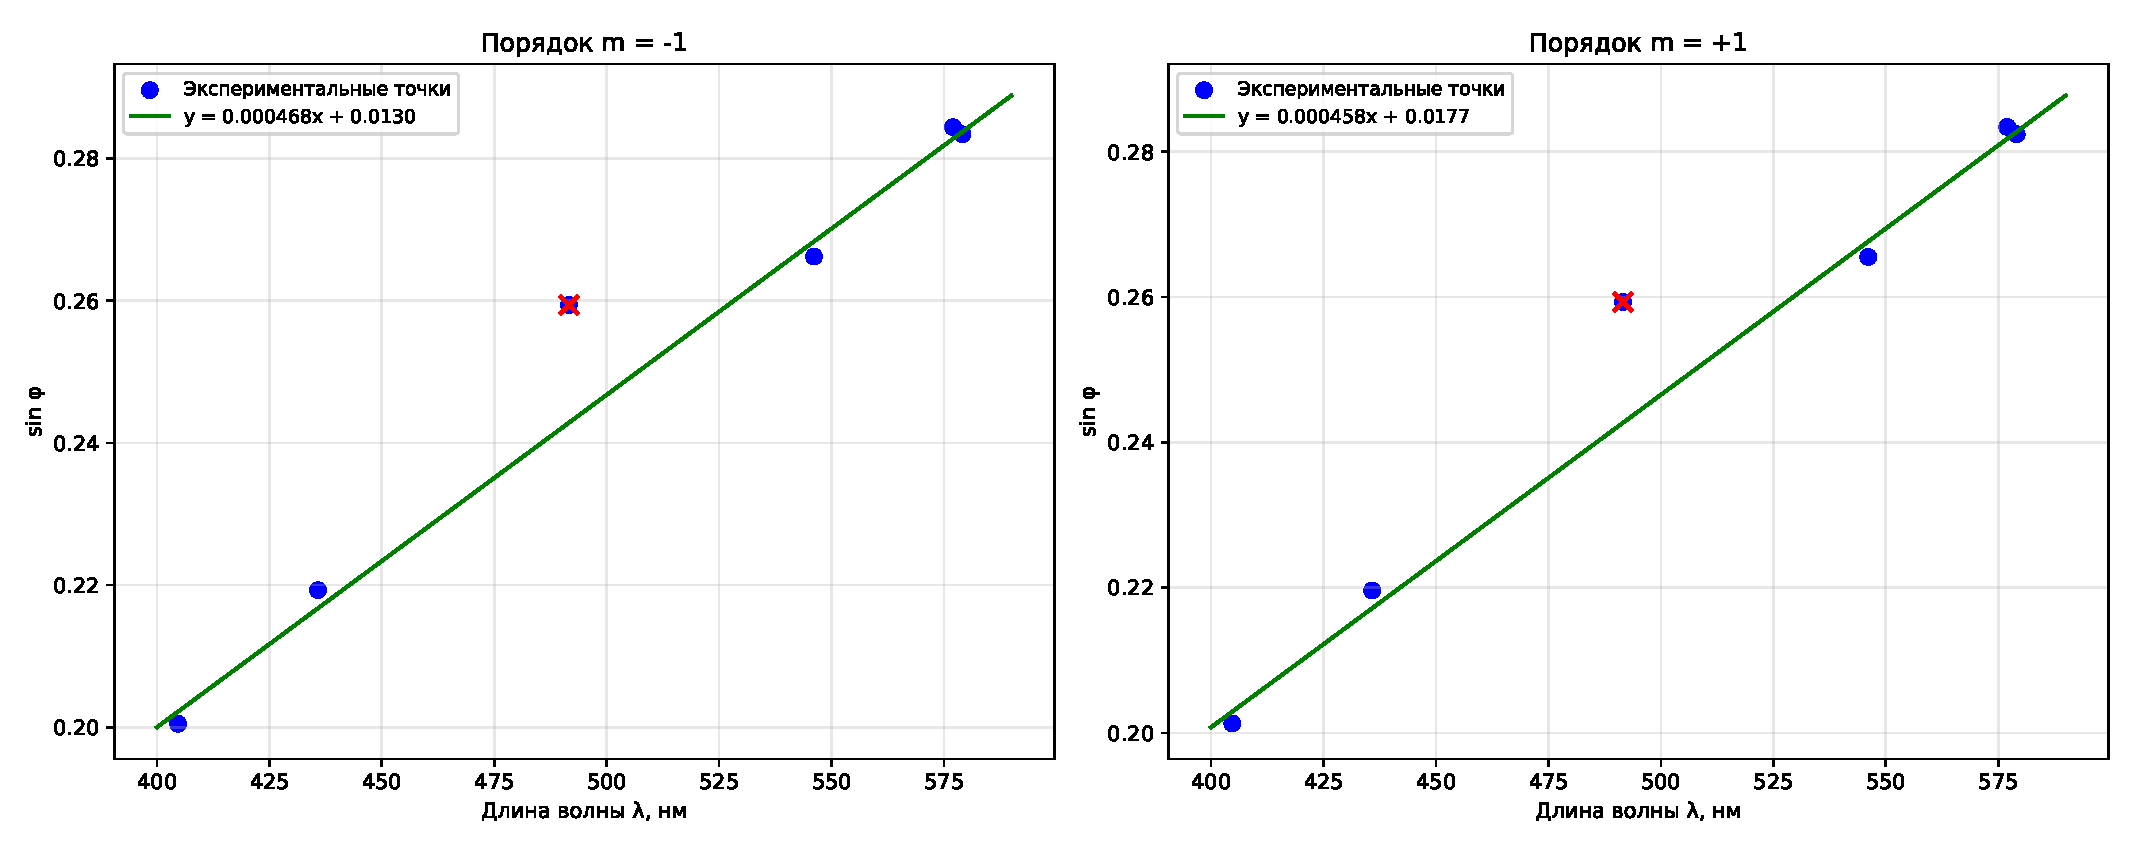
\includegraphics[width=1\textwidth]{sin.pdf}
    % \fbox{\parbox{0.8\textwidth}{\vspace{2cm}\centering \textbf{[Место для вставки графика $D = f(m)$]}\vspace{2cm}}}
    \caption{Графики зависимости $\sin(\varphi_m)$ от длины волны}
\end{figure}

Поскольку $\sin(\varphi_m) = \dfrac{m}{d}\lambda$, m=1, из углов наклона $k_{-1} = (0,000468\pm0,000014)$ нм$^{-1}$ и $k_{+1} = (0,000458\pm0,000014)$ нм$^{-1}$ был определён период решётки: $d_{-1} = (2139\pm56)$ нм и $d_{+1} = (2185\pm52)$ нм, что близко к истинному значению $d = 1/N = 2000$ нм.

\vspace{0.4cm}












% Для определения угловой дисперсии были измерены угловые положения компонент жёлтого дублета во всех видимых положительных и отрицательных порядках. Была рассчитана экспериментальная дисперсия $D = \Delta \varphi / \Delta \lambda$ (в угловых секундах на ангстрем). Зависимость $D = f(m)$ была построена и сопоставлена с теоретической кривой, рассчитанной по формуле (\ref{eq:dispersion}) для средней длины волны дублета.

% \begin{figure}[H]
%     \centering
%     % \includegraphics[width=0.8\textwidth]{dispersion_graph.png}
%     \fbox{\parbox{0.8\textwidth}{\vspace{2cm}\centering \textbf{[Место для вставки графика $D = f(m)$]}\vspace{2cm}}}
%     \caption{Зависимость угловой дисперсии от порядка спектра.}
%     \label{fig:dispersion}
% \end{figure}

% Для оценки аппаратной разрешающей способности была измерена угловая ширина одной из линий жёлтого дублета (по нулям интенсивности) в нескольких порядках. Аппаратная полуширина $\delta \lambda$ была рассчитана, после чего значение $R$ было определено по формуле (\ref{eq:resolving_exp}). Было оценено число эффективно работающих штрихов $N_{\text{эфф}}$ и размер освещённой области решётки.



\subsection*{3. Угловая дисперсия решётки}

Для определения угловой дисперсии решётки рассматривался жёлтый дублет $\lambda_1 = 577{,}0$ нм, $\lambda_2 = 579{,}1$ нм с разностью длин волн $\Delta\lambda = 2{,}1$ нм.

\subsection*{Экспериментальная угловая дисперсия}

Экспериментальная угловая дисперсия вычисляется по формуле:
\begin{equation}
    D_{\text{эксп}} = \frac{\Delta\varphi}{\Delta\lambda},
\end{equation}
где $\Delta\varphi$ -- угловое расстояние между компонентами дублета.

\begin{table}[h]
\centering
\begin{tabular}{|c|c|c|c|c|}
\hline
$m$ & $\varphi_1$ (577,0 нм) & $\varphi_2$ (579,1 нм) & $\Delta\varphi$, '' & $D_{\text{эксп}}$, ''/\AA \\
\hline
$+1$ & $163^\circ 28' 26''$ & $163^\circ 24' 24''$ & 244 & 11,62 \\
\hline
$-1$ & $197^\circ 01' 49''$ & $197^\circ 05' 40''$ & 240 & 11,43 \\
\hline
$+2$ & $145^\circ 00' 41''$ & $145^\circ 09' 39''$ & 538 & 25,62 \\
\hline
$-2$ & $215^\circ 38' 20''$ & $215^\circ 46' 39''$ & 499 & 23,76 \\
\hline
\end{tabular}
\caption{Угловые координаты жёлтого дублета и расчёт дисперсии}

\end{table}

\subsection*{Теоретическая угловая дисперсия}

Теоретическая зависимость рассчитывается по формуле:
\begin{equation}
    D_{\text{теор}} = \frac{m}{d\cos\varphi_m} = \frac{m}{\sqrt{d^2 - m^2\lambda^2}},
\end{equation}
где $\lambda = 578{,}05$ нм -- средняя длина волны дублета.

Углы дифракции $\varphi_m$ находились из формулы решётки $d\sin\varphi_m = m\lambda$:
\begin{itemize}
    \item $|m| = 1$: $\varphi_1 = \arcsin\left(\frac{578{,}05}{2000}\right) \approx 16{,}76^\circ$
    \item $|m| = 2$: $\varphi_2 = \arcsin\left(\frac{2\cdot 578{,}05}{2000}\right) \approx 35{,}25^\circ$
\end{itemize}

\begin{table}[h]
\centering
\caption{Сравнение экспериментальной и теоретической дисперсии}
\begin{tabular}{|c|c|c|c|}
\hline
$m$ & $\varphi_m$ (теор.) & $D_{\text{эксп}}$, ''/\AA & $D_{\text{теор}}$, ''/\AA \\
\hline
$\pm 1$ & $16{,}76^\circ$ & $11{,}53 \pm 0{,}10$ & 11,72 \\
\hline
$\pm 2$ & $35{,}25^\circ$ & $24{,}69 \pm 0{,}93$ & 24,89 \\
\hline
\end{tabular}
\end{table}


\begin{figure}[H]
    \centering
    
\includegraphics[width=0.9\textwidth]{3.pdf}
    % \fbox{\parbox{0.8\textwidth}{\vspace{3cm}\centering \textbf{[Место для графика $D = f(m)$]}\vspace{3cm}}}
    \caption{Зависимость угловой дисперсии от порядка спектра ($d = 2{,}00$ мкм, $\lambda = 578$ нм)}
    \label{fig:dispersion}
\end{figure}

Из графика видно, что экспериментальные значения дисперсии для $|m| = 1$ и $|m| = 2$ хорошо согласуются с теоретической зависимостью.
%     \item Относительное расхождение не превышает 2\%, что укладывается в погрешность измерений угловых координат.
%     \item Линейный рост дисперсии с порядком $m$ подтверждает справедливость формулы $D \propto m$.
%     \item Небольшое различие между положительными и отрицательными порядками объясняется погрешностью юстировки решётки и асимметрией оптической системы.
% \end{itemize}

% \textbf{Вывод:} Экспериментально подтверждена теоретическая зависимость угловой дисперсии от порядка спектра. Для решётки с периодом $d = 2{,}00$ мкм дисперсия составляет $\sim 11{,}5$ ''/\AA\ в первом порядке и $\sim 24{,}7$ ''/\AA\ во втором порядке.












\subsection*{4. Определение разрешающей способности решётки}

Для исследования была выбрана жёлтая линия с длиной волны $\lambda = 577{,}0$ нм

% \subsection*{Расчёт углов дифракции}

Углы дифракции рассчитываются как отклонение от нулевого порядка:
\begin{equation}
    \varphi_m = |\varphi_{\text{изм}} - \varphi_0|
\end{equation}

\begin{table}[H]
\centering

\begin{tabular}{|c|c|c|c|}
\hline
Порядок $m$ & Измеренный угол & $\varphi_m$ & $\varphi_m$ (сек) \\
\hline
$-1$ & $163^\circ 20' 31{,}5''$ & $16^\circ 39' 28{,}5''$ & 59 968 \\
\hline
$+1$ & $196^\circ 53' 27''$ & $16^\circ 53' 27''$ & 60 807 \\
\hline
$-2$ & $145^\circ 11' 8''$ & $34^\circ 48' 52''$ & 125 332 \\
\hline
$+2$ & $215^\circ 39' 28{,}5''$ & $35^\circ 39' 28{,}5''$ & 128 368 \\
\hline
\end{tabular}
\caption{Угловые координаты и углы дифракции}
\end{table}

% \subsection*{Экспериментальная разрешающая способность}

Разрешающая способность определяется как
\begin{equation}
    R_{\text{эксп}} = \frac{\varphi}{\delta\varphi}
\end{equation}

где $\delta\varphi$ -- угловая ширина спектральной линии.

\begin{table}[H]
\centering

\begin{tabular}{|c|c|c|c|c|}
\hline
$m$ & $\varphi$ (сек) & $\delta\varphi$ (сек) & $R_{\text{эксп}}$ & $N_{\text{эфф}} = R/|m|$ \\
\hline
$-1$ & 59 968 & 27 & 2 221 & 2 221 \\
\hline
$+1$ & 60 807 & 30 & 2 027 & 2 027 \\
\hline
$-2$ & 125 332 & 60 & 2 089 & 1 045 \\
\hline
$+2$ & 128 368 & 51 & 2 517 & 1 259 \\
\hline
\end{tabular}
\caption{Расчёт разрешающей способности}
\end{table}

Для расчётов были взяты средние значения:

Для первого порядка:
\begin{equation}
    R_1 = \frac{2221 + 2027}{2} \approx 2124, \quad 
    N_1 \approx 2124 \text{ штрихов}
\end{equation}

Для второго порядка:
\begin{equation}
    R_2 = \frac{2089 + 2517}{2} \approx 2303, \quad 
    N_2 = \frac{2303}{2} \approx 1152 \text{ штриха}
\end{equation}

\subsection*{Размер освещённой части решётки}

При 500 штр/мм размер освещённой области:
\begin{equation}
    L = \frac{N_{\text{эфф}}}{500 \text{ штр/мм}}
\end{equation}

\begin{itemize}
    \item Для $m = \pm 1$: $L_1 = \frac{2124}{500} \approx 4{,}25$ мм
    \item Для $m = \pm 2$: $L_2 = \frac{1152}{500} \approx 2{,}30$ мм
\end{itemize}

% \subsection*{Сравнение с теоретической разрешающей способностью}

Теоретическая разрешающая способность $R_{\text{теор}} = m \cdot N$, где $N$ -- полное число штрихов на решётке. Решётка имела размеры приблизительно 5$\times$5 см, так что $R_{\text{теор}} \sim 25000$, что существенно больше эффективной разрешающей способности.

% \textbf{Примечание:} Различие в оценках $N_{\text{эфф}}$ для разных порядков может быть связано с:
% \begin{itemize}
%     \item Неравномерностью освещения решётки
%     \item Уменьшением эффективной апертуры в высших порядках
%     \item Погрешностями измерения угловой ширины линий
% \end{itemize}

% \subsection*{Итоговые результаты}

% \begin{itemize}
%     \item Экспериментальная разрешающая способность (для $m=1$): $R \approx 2124$
%     \item Число эффективно работающих штрихов: $N_{\text{эфф}} \approx 2100$
%     \item Размер освещённой части решётки: $L \approx 4{,}2$ мм
%     \item Теоретическая разрешающая способность (при полном освещении): $R_{\text{теор}} = m \cdot N_{\text{полн}}$
% \end{itemize}

% \textbf{Вывод:} В эксперименте эффективно работает только часть решётки ($\sim 4$ мм из полной ширины), что ограничивает разрешающую способность установки.









% \subsection*{3. Зависимость разрешающей силы от ширины пучка}
% Зрительная труба была настроена на чёткое наблюдение жёлтого дублета. С помощью дополнительной щели с микрометрическим винтом было определено нулевое положение (момент полного закрытия). Измерение было повторено трижды при плавном открытии щели для устранения люфта и повышения точности отсчёта.

% Дополнительная щель была установлена на объективе коллиматора. Ширина пучка была плавно уменьшена до достижения предельного визуального разрешения компонент жёлтого дублета. Показания микрометрического винта, соответствующие критической ширине пучка, были зафиксированы. На основании измеренной разности длин волн дублета ($\Delta \lambda \approx 20$ Å) была оценена экспериментальная разрешающая способность $R$ в данном режиме. По формуле $R = m N$ было рассчитано число эффективно работающих штрихов $N$, после чего был определён фактический размер освещённой части решётки и число штрихов на миллиметр.






\subsection*{5. Расчёт порядка спектра для наложения линий}

Условие наложения спектральных линий разных порядков:
\begin{equation}
    d \sin \varphi = m_1 \lambda_1 = m_2 \lambda_2
\end{equation}

\noindent Длины волн из описания: жёлтая $\lambda_{\text{ж}} = 579{,}1$ нм, синяя $\lambda_{\text{ф}} = 435{,}8$ нм


\begin{equation}
    \frac{m_{\text{с}}}{m_{\text{ж}}} = \frac{\lambda_{\text{ж}}}{\lambda_{\text{с}}} = \frac{579{,}1}{435{,}8} \approx 1{,}329 \approx \frac{4}{3}
\end{equation}

\noindent Отсюда: $m_{\text{ж}} = 3$, $m_{\text{с}} = 4$

\begin{itemize}
    \item $m_{\text{ж}} = 3$: $3 \cdot 579{,}1 = 1737{,}3$ нм
    \item $m_{\text{с}} = 4$: $4 \cdot 435{,}8 = 1743{,}2$ нм
\end{itemize}

\noindent Разница: $\Delta = 1743{,}2 - 1737{,}3 = 5{,}9$ нм -- меньше ширины спектральной линиии, следовательно, наложение будет наблюдаться в 3-м порядке для жёлтой линии и 4-м порядке для синей линии.





\section*{6. Зависимость разрешающей силы от ширины пучка}

В данном эксперименте снова рассматривался жёлтый дублет: $\lambda \approx 578$ нм, $\Delta\lambda = 2{,}1$ нм в порядках спектра: $m = \pm1$
Для него была измерена критическая ширина щели (предельное разрешение):
    \begin{itemize}
        \item Для $m = -1$: $w_{-1} = 1{,}00$ мм
        \item Для $m = +1$: $w_{+1} = 0{,}84$ мм
    \end{itemize}
Средняя ширина: $\overline{w} = 0{,}92$ мм.


\subsection*{Расчёт разрешающей способности}

Разрешающая способность определяется как:
\begin{equation}
    R = \frac{\lambda}{\delta\lambda}
\end{equation}

При предельном разрешении жёлтого дублета минимальная разрешаемая разность длин волн равна разности компонент дублета: $\delta\lambda = \Delta\lambda = 2{,}1$ нм.

\begin{equation}
    R_{\text{эксп}} = \frac{578\text{ нм}}{2{,}1\text{ нм}} \approx 275
\end{equation}

\subsection*{Число эффективно работающих штрихов}

Из формулы разрешающей способности решётки:
\begin{equation}
    R = mN \quad \Rightarrow \quad N = \frac{R}{|m|} = \frac{275}{1} = 275 \text{ штрихов}
\end{equation}

\subsection*{Размер освещённой части решётки}

При периоде решётки $d = 2{,}00$ мкм (500 штр/мм) размер освещённой области:
\begin{equation}
    L = N \cdot d = 275 \cdot 2{,}00\text{ мкм} = 550\text{ мкм} = 0{,}55\text{ мм}
\end{equation}

\subsection*{Число штрихов на миллиметр}

Экспериментально определённое число штрихов на 1 мм:
\begin{equation}
    n = \frac{N}{L} = \frac{275}{0{,}92\text{ мм}} \approx 300 \text{ штр/мм}
\end{equation}

% Или, используя паспортное значение периода $d = 2{,}00$ мкм:
% \begin{equation}
%     n_0 = \frac{1}{d} = \frac{1}{2{,}00\text{ мкм}} = 500 \text{ штр/мм}
% \end{equation}

% \subsection*{Анализ результатов}

% \begin{itemize}
%     \item Разрешающая способность при ограничении ширины пучка: $R \approx 275$
%     \item Число эффективно работающих штрихов: $N \approx 275$
%     \item Теоретический размер освещённой области: $L_{\text{теор}} = 0{,}55$ мм
%     \item Измеренная средняя ширина щели: $\overline{w} = 0{,}92$ мм
% \end{itemize}

% \textbf{Примечание:} Различие между шириной щели ($0{,}92$ мм) и расчётным размером освещённой области ($0{,}55$ мм) объясняется тем, что не вся ширина щели эффективно используется для формирования пучка из-за апертуры коллиматора и геометрических факторов оптической схемы.

% \textbf{Вывод:} Экспериментально подтверждена зависимость разрешающей способности от ширины освещающего пучка. При сужении щели уменьшается число эффективно работающих штрихов, что приводит к снижению разрешающей способности до критического значения $R \approx 275$, при котором ещё возможно визуальное разделение компонент жёлтого дублета.







\section*{Выводы}


\begin{enumerate}
    \item Были измерены угловые координаты спектральных линий ртутной лампы в порядках $m = \pm 1$. Построены зависимости $\sin\varphi_m(\lambda)$, по угловым коэффициентам которых определён период решётки: $d_{-1} = (2139 \pm 56)$ нм и $d_{+1} = (2185 \pm 52)$ нм. Полученные значения близки к истинному значению. %в пределах погрешности.

    \item Экспериментально определена угловая дисперсия для жёлтого дублета ($\lambda = 577{,}0$ нм и $579{,}1$ нм) в порядках $|m| = 1, 2$. Значения $D_{\text{эксп}} = 11{,}53 \pm 0{,}10$ ''/\AA\ ($|m|=1$) и $D_{\text{эксп}} = 24{,}69 \pm 0{,}93$ ''/\AA\ ($|m|=2$) хорошо описываются теоретической зависимостью $D = m/(d\cos\varphi_m)$.

    \item Рассчитана разрешающая способность установки: $R \approx 2124$ для первого порядка спектра. Оценено число эффективно работающих штрихов $N_{\text{эфф}} \approx 2100$ и размер освещённой области решётки $L \approx 4{,}2$ мм. Полученное значение $R$ существенно меньше теоретического максимума ($R_{\text{теор}} \sim 25000$), что объясняется ограниченной апертурой пучка и конечной шириной входной щели.

    % \item Рассчитан порядок перекрытия спектров: наложение синей линии ($435{,}8$ нм) 4-го порядка на жёлтую линию ($579{,}1$ нм) 3-го порядка подтверждено расчётом ($\Delta = 5{,}9$ нм $<$ ширины линии).

    \item Исследовано влияние ширины пучка на разрешающую способность. При сужении щели до критической ширины $\overline{w} = 0{,}92$ мм разрешающая способность снижается до $R \approx 275$, что соответствует $N \approx 275$ эффективно работающим штрихам. Подтверждена прямая зависимость $R \propto N$.
\end{enumerate}

\end{document}